\documentclass[11pt]{article}
\usepackage[margin=1in]{geometry}
\usepackage{graphicx}
\usepackage{booktabs}
\usepackage{amsmath,amssymb}
\usepackage[numbers]{natbib}
\usepackage[colorlinks=true,linkcolor=blue,citecolor=blue,urlcolor=blue]{hyperref}
\usepackage{microtype}

\title{Forecasting Conformal Coverage Loss under Model Compression}
\author{Satyawan Singh\\
\small University of Leicester (MSc AI, 2025); independent researcher\\
\small \texttt{satyawansinghinuk@gmail.com}}
\date{August 2026}

\begin{document}
\maketitle

\begin{abstract}
Deployed classifiers are routinely compressed after calibration: a model whose
conformal guarantee was calibrated in FP32 ships with quantized weights. We show
empirically that this silently invalidates the guarantee, and, more usefully,
that the coverage loss is \emph{forecastable before deployment}. Treating
post-training quantization as a computable shift of the nonconformity-score
distribution, an elementary Kolmogorov/total-variation argument upper-bounds the
coverage deficit under stale calibration by the distance between the reference
and deployed score distributions, both measurable on the labeled calibration set
already in hand. Across 2 datasets $\times$ 2 architectures $\times$ 5
bit-widths (60 runs), the bound held in every run, and in the damage regime on
peaked score distributions it is nearly tight: at 4-bit and 3-bit precision the
measured deficit matched the total-variation distance to within 0.003. We
further characterize what recalibration can and cannot repair: validity is
restored at every precision tested, including models degraded to 47.8\%
accuracy, while informativeness collapses past an architecture-dependent
precision knee (mean prediction-set size 0.91 at 8-bit versus 5.6--9.4 classes
at 3-bit). A deployment corollary under simulated sensor drift shows that
refreshing only the calibration scores (kilobytes; no retraining) maintains
validity where launch calibration decays from 90.7\% to 20.9\% coverage, with
prediction-set growth acting as the model-health signal. All results are
reproducible from public code and raw data.
\end{abstract}

\section{Introduction}

Split conformal prediction wraps any classifier with a distribution-free
guarantee: prediction sets that contain the true label with probability at
least $1-\alpha$ under exchangeability \citep{vovk2005,papadopoulos2002,angelopoulos2023}.
The guarantee is calibrated on held-out data using the model's nonconformity
scores. In deployment practice, however, the model that ships is rarely the
model that was calibrated. Post-training quantization (PTQ), pruning, and
distillation intervene between calibration and deployment, particularly in
resource-constrained settings (mobile, embedded, onboard spacecraft) where
compression is mandatory.

This paper asks a narrow question with practical consequences: \emph{what does
compression do to a conformal guarantee calibrated on the uncompressed model,
and can the damage be predicted in advance?} Our answers:

\begin{enumerate}
  \item \textbf{Stale calibration silently undercovers} (Section~\ref{sec:break}).
  Reusing FP32 calibration on an INT8 deployment undercovers at every miscoverage
  level tested, while accuracy is essentially unchanged, the failure is
  invisible to accuracy monitoring.
  \item \textbf{The loss is forecastable} (Sections~\ref{sec:bound},~\ref{sec:tight}).
  The coverage deficit is upper-bounded by the total-variation (TV) distance
  between reference and deployed score distributions on the calibration set,
  a quantity computable on the ground, before deployment, with no new data. The
  bound is elementary; the contribution is empirical: it held in 60/60 runs
  across datasets, architectures, and bit-widths, and in the damage regime on
  peaked score distributions it is nearly an equality.
  \item \textbf{Recalibration restores validity but not informativeness}
  (Section~\ref{sec:eff}). Coverage returns to target at every precision, even
  for badly damaged models; mean prediction-set size, by contrast, exhibits a
  sharp knee in precision, one full bit earlier for MobileNetV3 than for
  ResNet18. Set size on calibration data is therefore the natural acceptance
  test for a compressed artifact.
  \item \textbf{Deployment corollary} (Section~\ref{sec:drift}): under
  progressive sensor drift, periodically refreshing the calibration scores
  (200 labeled samples per refresh; no retraining) largely preserves validity,
  and set-size growth signals when the model itself, rather than its
  calibration, requires intervention.
\end{enumerate}

\section{Related work}

\textbf{Conformal prediction under shift.} \citet{barber2023} bound the
coverage gap of conformal prediction beyond exchangeability by the total
variation between calibration and test distributions, with weighted variants;
subsequent work refines such bounds under Wasserstein and other metrics. Our
setting is complementary: the data remain exchangeable, and the shift is
induced in the \emph{score function} by compressing the model. We instantiate
the same style of bound for this self-inflicted, fully measurable shift and
characterize its tightness empirically.

\textbf{Uncertainty for onboard and remote-sensing models.}
\citet{marchante2025} study conformal prediction for onboard Earth observation
under domain shift with weighted conformal methods, and the same group proposes
class-conditional randomized smoothing against structured spectral corruptions
\citep{marchante2025copa}. These address input-side shift; neither considers
compression of the model itself, which is the axis studied here. We view the
two as composable layers of the same deployment problem.

\textbf{Compression and uncertainty.} A recent benchmark studies uncertainty
under compression for large language models \citep{compressionUQ2026},
reporting threshold-like degradation. Our vision results differ: on EuroSAT
and CIFAR-10 the collapse of stale-calibration coverage is smooth and tracks
the measured score shift (Section~\ref{sec:scaling}), and we additionally
study the stale-versus-recalibrated distinction and set-size efficiency, which
that benchmark does not address.

\section{Setup and the forecasting bound}\label{sec:bound}

Let $f_{\mathrm{ref}}$ be the calibrated (reference) classifier and
$f_{q}$ its compressed deployment. Split conformal prediction with the LAC
score $s(x,y) = 1 - p_y(x)$ computes the threshold $\hat{q}$ as the
$\lceil (1-\alpha)(n+1)\rceil/n$ empirical quantile of calibration scores
$S^{\mathrm{ref}}_i = s_{\mathrm{ref}}(X_i, Y_i)$, giving
$\mathbb{P}(S^{\mathrm{ref}} \le \hat{q}) \ge 1-\alpha$ on exchangeable data.
If deployment instead evaluates $f_q$ while retaining $\hat q$ (\emph{stale
calibration}), realized coverage is $\mathbb{P}(S^{q} \le \hat{q})$, and the
deficit obeys
\begin{equation}
(1-\alpha) - \mathbb{P}(S^{q} \le \hat{q})
\;\le\; \sup_t \left| F_{S^{\mathrm{ref}}}(t) - F_{S^{q}}(t) \right|
\;=\; d_K(S^{\mathrm{ref}}, S^{q})
\;\le\; d_{TV}(S^{\mathrm{ref}}, S^{q}),
\label{eq:bound}
\end{equation}
up to the usual finite-sample slack in the calibration quantile. The
inequality itself is elementary; its value is operational. Because compression
is applied by the deployer, both score distributions are computable on the
\emph{same labeled calibration set}: quantize, re-score, estimate
$d_{TV}$ (we use 1000-bin histograms on $[0,1]$). The result is a pre-flight
forecast: an upper bound on the coverage that will be lost if calibration is
not refreshed. The empirical questions are whether the bound holds under
estimation error and how tight it is; the remainder of the paper measures
this.

\section{Experiments}

\textbf{Protocol.} Datasets: EuroSAT RGB \citep{helber2019} (27{,}000 tiles,
10 classes; 70/15/15 train/calibration/test) and CIFAR-10 \citep{krizhevsky2009}.
Architectures: ResNet18 \citep{he2016} and MobileNetV3-Small
\citep{howard2019}, ImageNet-initialized, 12 epochs AdamW. Compression:
symmetric per-channel weight quantization to $b \in \{8,6,4,3,2\}$ bits
(simulated PTQ: quantized values, FP32 arithmetic), plus production INT8
(FX-graph PTQ) for Section~\ref{sec:break}. Multi-seed throughout; error bars
are standard deviations over seeds. Code, raw results, and exact environment
are public; a fresh-clone reproduction test recovers the reported numbers
exactly.\footnote{\url{https://github.com/ss1738/euroSAT-CNN-landcover}}

\subsection{Stale calibration silently undercovers}\label{sec:break}

On EuroSAT/ResNet18 with production INT8 PTQ (20 seeds), accuracy is
essentially unchanged (98.13\% $\to$ 98.03\%) while stale-calibration
coverage falls below target at every level tested: $88.8 \pm 0.8\%$ against a
90\% target ($\alpha{=}0.10$), $94.4 \pm 0.6\%$ against 95\%, and
$83.0 \pm 0.8\%$ against 85\%, the gap growing with $\alpha$. Recalibrating
on the quantized model restores target coverage at all levels
($90.0 \pm 0.7\%$, $94.9 \pm 0.5\%$, $84.9 \pm 0.6\%$). The practical rule is
stark: \emph{calibrate the artifact that ships, not the model that trained}.

\subsection{Coverage collapse is smooth and tracks the score shift}\label{sec:scaling}

Sweeping precision on EuroSAT/ResNet18 (5 seeds;
Figure~\ref{fig:scaling}): stale-calibration coverage falls monotonically,
$89.8\%$ (8-bit), $88.9\%$ (6-bit), $66.5\%$ (4-bit), $11.6\%$ (3-bit),
$1.9\%$ (2-bit) against a 90\% target, tracking the relative weight
perturbation (1.1\%, 4.4\%, 19.6\%, 42.2\%, 75.2\%) and the mean absolute
probability shift. We observe no threshold effect: degradation is gradual in
the measured shift, in contrast to the threshold-like behaviour reported for
LLMs \citep{compressionUQ2026}. Recalibration restores target coverage at
\emph{every} precision, including a 3-bit model at 47.8\% accuracy (coverage
$89.7\%$) and a 2-bit model at 10.3\% accuracy (coverage 100\%, attained by
prediction sets growing toward all classes, see Section~\ref{sec:eff}).

\begin{figure}[t]
\centering
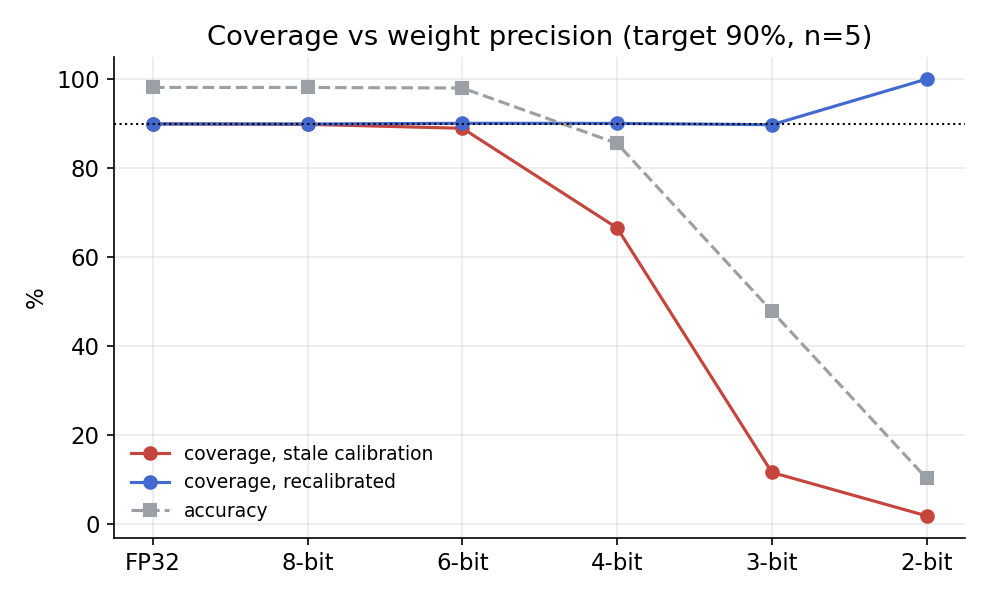
\includegraphics[width=0.62\linewidth]{figures/scaling_law.png}
\caption{Coverage versus weight precision (EuroSAT/ResNet18, $n{=}5$ seeds,
target 90\%). Stale calibration (red) collapses smoothly; recalibration
(blue) restores validity at every precision while accuracy (gray) falls.}
\label{fig:scaling}
\end{figure}

\subsection{The bound holds and is nearly tight in the damage regime}\label{sec:tight}

Figure~\ref{fig:tv} plots measured deficit against estimated
$d_{TV}(S^{\mathrm{ref}}, S^{q})$ per bit-width (5 seeds). At 8- and 6-bit
the bound is conservative (deficit 0.002 and 0.011 against TV 0.030 and
0.034). In the damage regime it is nearly an equality: deficit 0.235 against
TV 0.238 at 4-bit and 0.784 against 0.783 at 3-bit. The single nominal
violation (0.001 at 3-bit) is within histogram-estimation error of the TV
distance. Thus the forecast errs safe where damage is small and is
near-exact where it matters.

\begin{figure}[t]
\centering
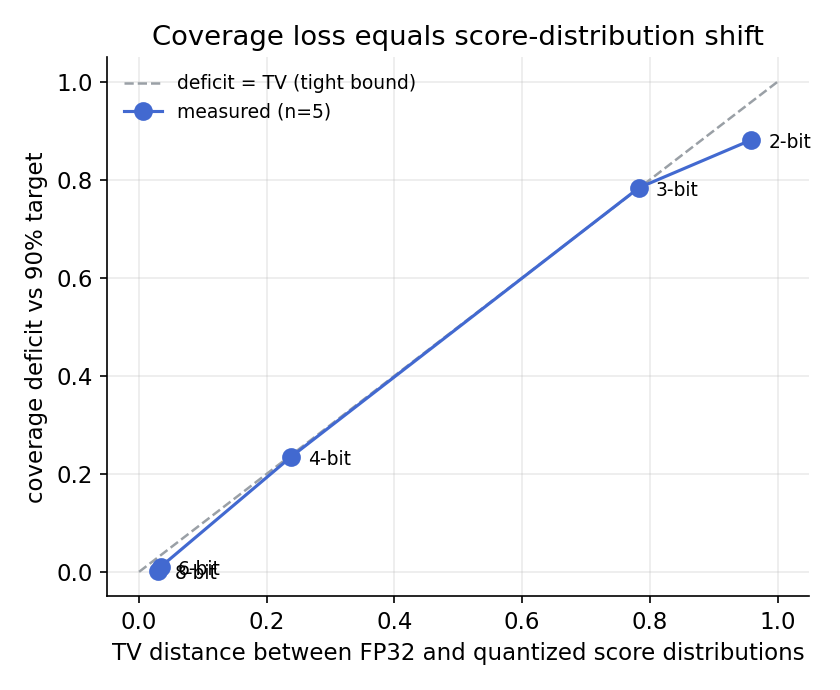
\includegraphics[width=0.5\linewidth]{figures/tv_bound.png}
\caption{Coverage deficit versus TV distance between reference and deployed
score distributions (EuroSAT/ResNet18). The dashed diagonal is
deficit $=$ TV.}
\label{fig:tv}
\end{figure}

\textbf{Generality.} Repeating the test over the full grid, \{EuroSAT,
CIFAR-10\} $\times$ \{ResNet18, MobileNetV3-Small\} $\times$
\{8,6,4,3,2\}-bit, 3 seeds each, the bound of Eq.~\eqref{eq:bound} held in
\textbf{60 of 60 runs} (Figure~\ref{fig:gen}). Tightness is systematic rather
than accidental: on EuroSAT, whose score distribution is strongly peaked
(high-confidence task), deficit approaches TV (e.g.\ 0.776 vs.\ 0.797,
ResNet18 at 3-bit); on CIFAR-10, with broader score distributions, the bound
is conservative (0.371 vs.\ 0.525). The forecast therefore never
underestimated the loss in our experiments and approaches equality precisely
on the peaked, high-accuracy regimes typical of deployed special-purpose
classifiers. A secondary observation with engineering value: MobileNetV3 is
markedly more quantization-fragile than ResNet18 (deficit 0.623 vs.\ 0.235 at
4-bit on EuroSAT), consistent with per-channel quantization of depthwise
convolutions; architecture choice is an assurance decision, not only an
accuracy one.

\begin{figure}[t]
\centering
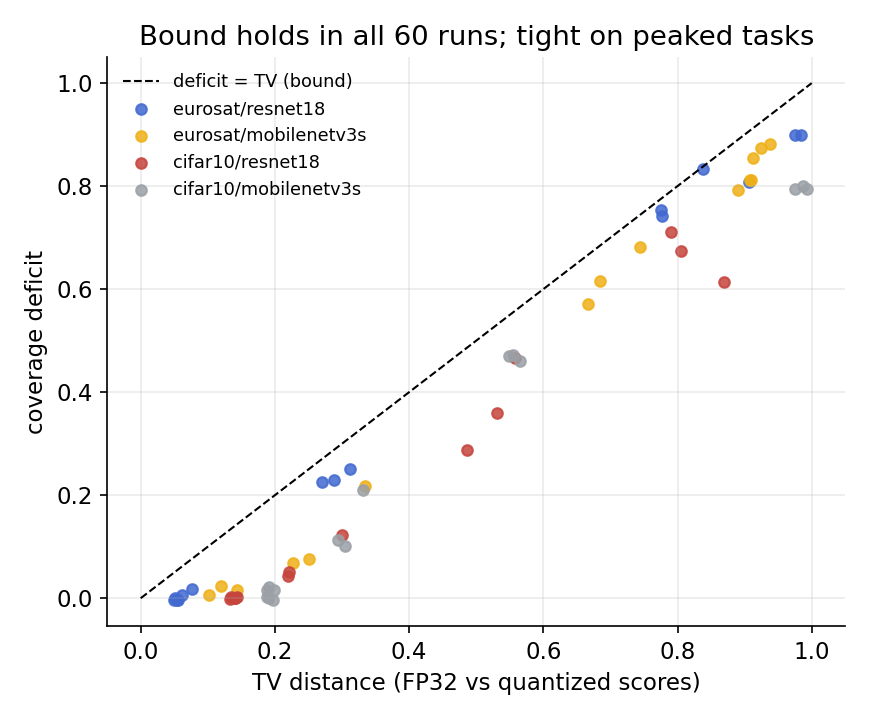
\includegraphics[width=0.52\linewidth]{figures/generality.png}
\caption{All 60 runs across the dataset $\times$ architecture $\times$
precision grid. Every point lies on or below the diagonal (bound holds);
peaked-task points hug it.}
\label{fig:gen}
\end{figure}

\subsection{Validity is recoverable; informativeness is not}\label{sec:eff}

Recalibration always restores coverage, but the guarantee can be honored
vacuously. Mean prediction-set size after recalibration
(Figure~\ref{fig:eff}) stays near one class down to 6-bit (0.91--1.24 across
the grid), passes a knee at 4-bit (1.14 for EuroSAT/ResNet18 but already 4.94
for EuroSAT/MobileNetV3), and explodes at 3-bit (5.2--9.4 classes),
saturating near all 10 classes at 2-bit. Validity and informativeness thus
separate cleanly under compression: the former is always repairable by
re-scoring, the latter has an architecture-dependent precision floor. Mean
set size on the calibration set is consequently a one-line acceptance test
for whether a compressed artifact is worth deploying.

\begin{figure}[t]
\centering
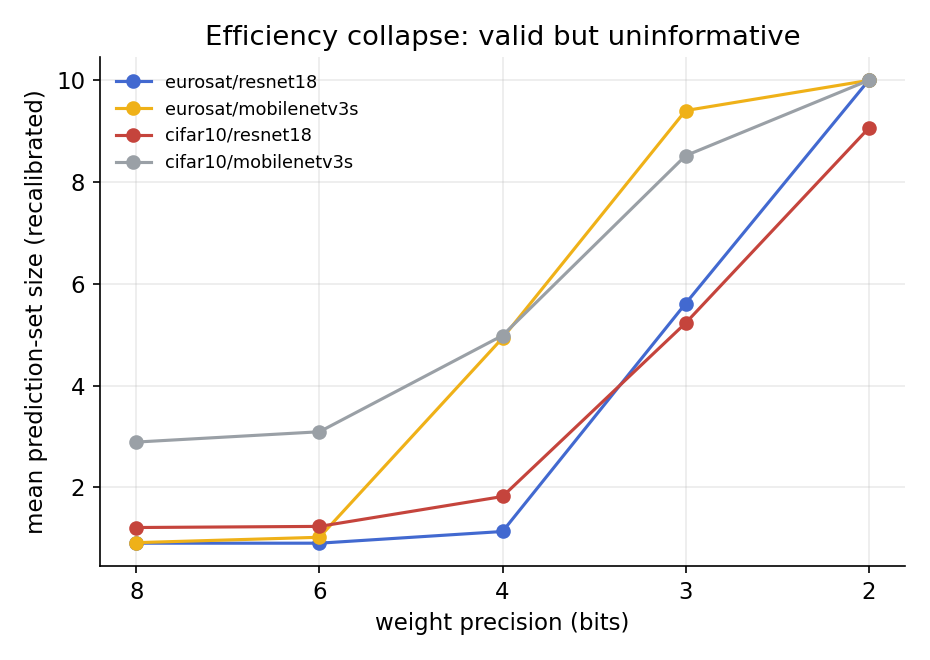
\includegraphics[width=0.55\linewidth]{figures/efficiency.png}
\caption{Mean recalibrated prediction-set size versus precision across the
grid: valid but uninformative below the knee.}
\label{fig:eff}
\end{figure}

\section{Deployment corollary: refresh the guarantee, not the model}\label{sec:drift}

Compression is one source of score shift; sensor drift over a mission is
another, and the same machinery applies. Under a simulated 24-week
progressive degradation (additive noise ramping to $\sigma{=}0.05$ and
brightness to $\times 1.35$; EuroSAT/ResNet18, 3 seeds,
Figure~\ref{fig:drift}), never-refreshed launch calibration decays from
90.7\% to 20.9\% coverage. Refreshing \emph{only the conformal scores} every
4 weeks, 200 labeled samples per refresh, kilobytes of storage, no
retraining or gradients, holds coverage at 81--87\% through end of test; a
12-week cadence is insufficient (54.0\% at week 23), so refresh rate must
track drift rate. Under the working refresh, mean set size grows from 0.91 to
6.65 as model accuracy falls from 97.8\% to 30.9\%: the guarantee remains
honest by becoming less informative, and set-size growth is precisely the
onboard signal that the model, not the calibration, now requires
intervention.

\begin{figure}[t]
\centering
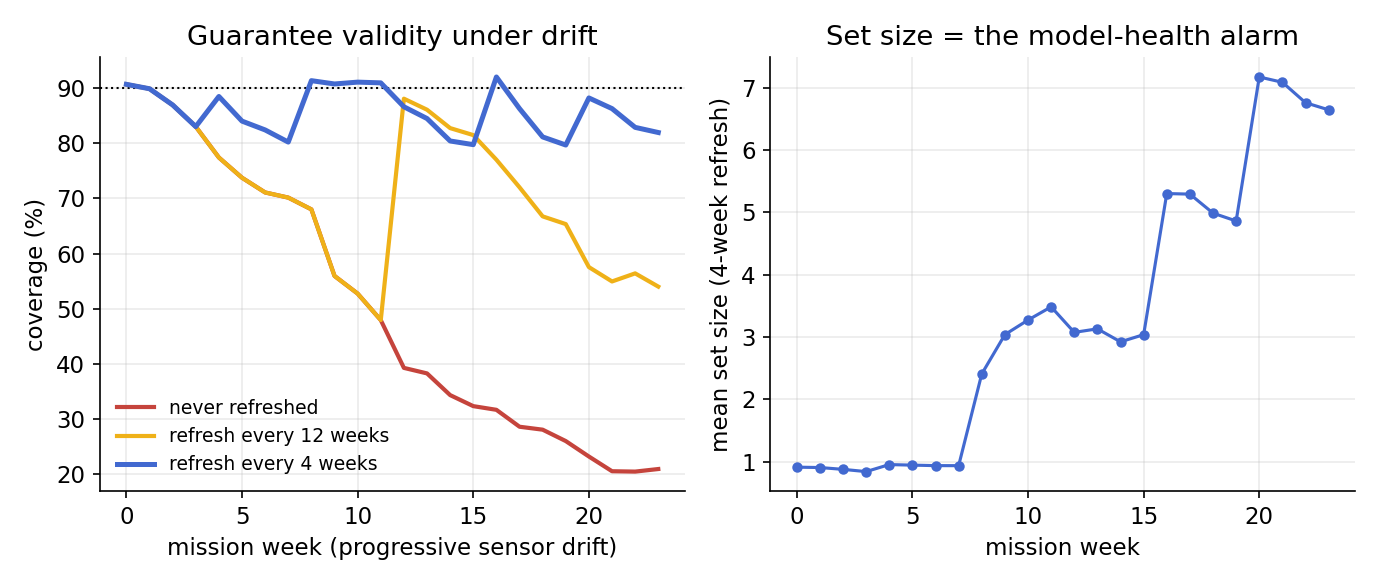
\includegraphics[width=0.75\linewidth]{figures/drift.png}
\caption{Simulated mission drift. Left: coverage under three maintenance
policies (target 90\%). Right: set size under the working policy is the
model-health signal.}
\label{fig:drift}
\end{figure}

\section{Limitations}

The bound in Eq.~\eqref{eq:bound} is elementary and one-directional; we claim
no new theory, only its instantiation, validation, and operational use for
compression. TV is estimated by histograms; at extreme damage (3-bit) the
estimator error is visible as a 0.001 nominal violation. Experiments cover
split conformal classification with the LAC score on two mid-scale vision
datasets and two architectures; regression, other scores, and
larger-scale models are untested. Quantization is simulated PTQ (quantized
weights, FP32 arithmetic) except where production INT8 is stated; activation
quantization is not studied. Drift is synthetic and the refresh policy
assumes access to small labeled batches. Findings on fault injection and
input-side monitoring from the same research programme are reported in the
repository rather than here.

\section{Conclusion}

A conformal guarantee does not survive model compression by default, but its
loss is not a surprise to be discovered in deployment: it is a number that
can be computed on the ground, from data already in hand, before the artifact
ships. Together with the recoverability of validity, the precision knee in
informativeness, and score-refresh as a maintenance policy, this yields a
practical qualification recipe for compressed classifiers under
distribution-free guarantees.

\bibliographystyle{plainnat}
\begin{thebibliography}{12}

\bibitem[Vovk et al.(2005)]{vovk2005}
V.~Vovk, A.~Gammerman, and G.~Shafer.
\newblock \emph{Algorithmic Learning in a Random World}.
\newblock Springer, 2005.

\bibitem[Papadopoulos et al.(2002)]{papadopoulos2002}
H.~Papadopoulos, K.~Proedrou, V.~Vovk, and A.~Gammerman.
\newblock Inductive confidence machines for regression.
\newblock In \emph{ECML}, 2002.

\bibitem[Angelopoulos and Bates(2023)]{angelopoulos2023}
A.~N. Angelopoulos and S.~Bates.
\newblock Conformal prediction: A gentle introduction.
\newblock \emph{Foundations and Trends in Machine Learning}, 2023.

\bibitem[Barber et al.(2023)]{barber2023}
R.~F. Barber, E.~J. Cand\`es, A.~Ramdas, and R.~J. Tibshirani.
\newblock Conformal prediction beyond exchangeability.
\newblock \emph{Annals of Statistics}, 51(2):816--845, 2023.

\bibitem[Marchante~Arjona et al.(2025a)]{marchante2025}
L.~Marchante~Arjona, P.~Bhattacharjee, and P.~Jung.
\newblock Onboard conformal prediction for domain shift in Earth observation.
\newblock In \emph{Proc. SPIE 13670, Sensors + Imaging}, 2025.

\bibitem[Marchante~Arjona et al.(2025b)]{marchante2025copa}
L.~Marchante~Arjona, P.~Bhattacharjee, and P.~Jung.
\newblock Class-conditional robust conformal prediction for structured
  perturbations.
\newblock In \emph{Proc. COPA, PMLR v266}, 2025.

\bibitem[Anonymous(2026)]{compressionUQ2026}
Does compression preserve uncertainty? A benchmark for uncertainty
  quantification in compressed LLMs.
\newblock arXiv:2606.01850, 2026.

\bibitem[Helber et al.(2019)]{helber2019}
P.~Helber, B.~Bischke, A.~Dengel, and D.~Borth.
\newblock EuroSAT: A novel dataset and deep learning benchmark for land use
  and land cover classification.
\newblock \emph{IEEE JSTARS}, 2019.

\bibitem[Krizhevsky(2009)]{krizhevsky2009}
A.~Krizhevsky.
\newblock Learning multiple layers of features from tiny images.
\newblock Technical report, 2009.

\bibitem[He et al.(2016)]{he2016}
K.~He, X.~Zhang, S.~Ren, and J.~Sun.
\newblock Deep residual learning for image recognition.
\newblock In \emph{CVPR}, 2016.

\bibitem[Howard et al.(2019)]{howard2019}
A.~Howard et~al.
\newblock Searching for MobileNetV3.
\newblock In \emph{ICCV}, 2019.

\end{thebibliography}

\end{document}
